\documentclass[10pt,a4paper]{article}
\ifdefined\pdftexversion\pdfoutput=1\fi

\usepackage[a4paper,left=2.3cm,right=2.3cm,top=2.5cm,bottom=2.6cm]{geometry}
\usepackage{amsmath,amssymb}
\usepackage{graphicx}
\usepackage{booktabs}
\usepackage{caption}
\usepackage[table]{xcolor}
\usepackage[colorlinks=true,linkcolor=blue!55!black,
            citecolor=blue!55!black,urlcolor=blue!55!black]{hyperref}

\captionsetup{font=small,labelfont=bf,width=.94\textwidth}
\setlength{\parskip}{0pt}
\newcommand{\GB}{\mathrm{GB}}
\newcommand{\ext}{\mathrm{ext}}
\newcommand{\dd}{\mathrm{d}}
\newcommand{\aX}[1]{\href{https://arxiv.org/abs/#1}{arXiv:#1}}

% Every number below is read from the measurement, not typed here.
% Generated by make_figures.py from ../results/egb-extremality.json.
% Do not edit: every macro below is read from the measurement.

\newcommand{\Ncouplings}{13}
\newcommand{\Nstates}{356}
\newcommand{\Nresolution}{64}
\newcommand{\Nrefinedresolution}{96}
\newcommand{\Ncoarseresolution}{48}
\newcommand{\Npsiextzero}{3.141592534}
\newcommand{\Npsiextzerodev}{1.19\times 10^{-7}}
\newcommand{\Nmuzero}{2.196887831}
\newcommand{\Nmuzerodev}{4.56\times 10^{-11}}
\newcommand{\Nmasscoefficient}{2.196887831}
\newcommand{\Npsimin}{1.07149}
\newcommand{\Nymin}{0.1752}
\newcommand{\Nxmin}{0.1669}
\newcommand{\Nalphamin}{0.15}
\newcommand{\Npsilast}{1.44440}
\newcommand{\Nylast}{0.5112}
\newcommand{\Nxlast}{0.5001}
\newcommand{\Nxextlast}{0.4170}
\newcommand{\Nworstj}{1.000000}
\newcommand{\Nsigmagrowth}{4.8}
\newcommand{\Nhalfpsi}{1.3260}
\newcommand{\Nhalfx}{0.0871}
\newcommand{\Nsuppression}{2.93}
\newcommand{\Ngriderror}{1.30\times 10^{-2}}
\newcommand{\Noracledigits}{8}
\newcommand{\Noraclegood}{9}
\newcommand{\Noracletotal}{11}
\newcommand{\Noracleworst}{2.86\times 10^{-8}}
\newcommand{\Nperturbativezero}{0.634936}
\newcommand{\Nlocuszero}{0.63474}
\newcommand{\Nlocuszerodev}{1.95\times 10^{-4}}
\newcommand{\Nratiolow}{3.951}
\newcommand{\Nratiohigh}{4.028}
\newcommand{\Nrefinementpoints}{4}
\newcommand{\Nrefinementsteps}{5}
\newcommand{\Nlargestgap}{1.47\times 10^{-2}}
\newcommand{\Ntaufloor}{4.61\times 10^{-3}}
\newcommand{\Ntaubest}{3.34\times 10^{-6}}
\newcommand{\Ntensorworst}{9.76\times 10^{-9}}
\newcommand{\Nsmarrworst}{1.64\times 10^{-7}}
\newcommand{\Ncontrastworst}{2.56\times 10^{-5}}
\newcommand{\Ncontrastmu}{6.03\times 10^{-6}}
\newcommand{\Nrouteworst}{1.64\times 10^{-4}}
\newcommand{\Nrouteworstrel}{1.96\times 10^{-3}}
\newcommand{\Nroutetrapezoid}{8.76\times 10^{-4}}
\newcommand{\Nroutecumulative}{4.38\times 10^{-4}}
\newcommand{\Nmutotal}{0.6916}
\newcommand{\Nmassslope}{3.144521}
\newcommand{\Nmassslopedev}{2.93\times 10^{-3}}
\newcommand{\Nmassslopespread}{2.09\times 10^{-2}}
\newcommand{\Nstaticpsiworst}{2.60\times 10^{-9}}
\newcommand{\Nstaticmassworst}{3.20\times 10^{-11}}
\newcommand{\Nstaticentropyworst}{1.00\times 10^{-16}}
\newcommand{\Nstatictempworst}{1.08\times 10^{-13}}
\newcommand{\Nstaticcouplings}{7}
\newcommand{\Nvacuummassworst}{3.27\times 10^{-13}}
\newcommand{\Nfirstlawworst}{1.35\times 10^{-8}}
\newcommand{\Ngoonpencoworst}{4.84\times 10^{-8}}
\newcommand{\Nconditionworst}{5.4\times 10^{7}}
\newcommand{\Nconsistencypoints}{10}
\newcommand{\Nvacuumspin}{0.7}
\newcommand{\Ntailspreadworst}{1.31\times 10^{-8}}
\newcommand{\Ntailwindows}{$z\in[0.03,0.12]$ at degree $4$, $z\in[0.04,0.16]$ at degree $4$, $z\in[0.03,0.12]$ at degree $3$}
\newcommand{\Nminimumlow}{0.118}
\newcommand{\Nminimumhigh}{0.229}
\newcommand{\Nhorizonworst}{4.06\times 10^{-6}}
\newcommand{\Npublishedstationarity}{9.17\times 10^{-14}}
\newcommand{\Npublishedspin}{6.66\times 10^{-16}}
\newcommand{\Nvacuumj}{1.00000000}
\newcommand{\Njlast}{0.66328}
\newcommand{\Njlocusfirst}{0.98074}
\newcommand{\Njlocuslast}{0.47284}
\newcommand{\Ntlocusfirst}{0.32448}
\newcommand{\Ntlocusmin}{0.19519}
\newcommand{\Nalphalocusmin}{0.1}

% Table: the sign-change locus.
\newcommand{\Nlocustable}{%
  $0$ & $0.0000$ & $0.32448$ & $7.35\times 10^{-2}$ & $0.98074$ & $0.63474$ \\
  $0.02$ & $0.0247$ & $0.27982$ & $5.73\times 10^{-2}$ & $0.94334$ & $0.66943$ \\
  $0.05$ & $0.0629$ & $0.22716$ & $4.93\times 10^{-2}$ & $0.90205$ & $0.71070$ \\
  $0.1$ & $0.1240$ & $0.19519$ & $3.92\times 10^{-2}$ & $0.85537$ & $0.73172$ \\
  $0.2$ & $0.2331$ & $0.21922$ & $2.82\times 10^{-2}$ & $0.77828$ & $0.67959$ \\
  $0.5$ & $0.4829$ & $0.34262$ & $1.33\times 10^{-2}$ & $0.47284$ & $0.37294$ \\
}

% Table: the extremal branch.
\newcommand{\Nextremaltable}{%
  $0$ & $0.00000$ & $0.00000$ & $2.196888$ & $3.14159$ & $1.15\times 10^{-2}$ & $1.00000$ & $6.2832$ \\
  $0.005$ & $0.00479$ & $0.00510$ & $2.211579$ & $2.99094$ & $1.12\times 10^{-1}$ & $0.99005$ & $6.6686$ \\
  $0.01$ & $0.00984$ & $0.01042$ & $2.226279$ & $2.82456$ & $8.81\times 10^{-2}$ & $0.98026$ & $7.0685$ \\
  $0.02$ & $0.02072$ & $0.02165$ & $2.255058$ & $2.47283$ & $1.60\times 10^{-1}$ & $0.96156$ & $7.8933$ \\
  $0.035$ & $0.03843$ & $0.03946$ & $2.294438$ & $2.00066$ & $1.32\times 10^{-1}$ & $0.93691$ & $9.1213$ \\
  $0.05$ & $0.05689$ & $0.05758$ & $2.328017$ & $1.65908$ & $1.86\times 10^{-2}$ & $0.91671$ & $10.2781$ \\
  $0.075$ & $0.08775$ & $0.08711$ & $2.373482$ & $1.32597$ & $2.20\times 10^{-2}$ & $0.89050$ & $12.0267$ \\
  $0.1$ & $0.11787$ & $0.11521$ & $2.410729$ & $1.16621$ & $2.10\times 10^{-2}$ & $0.86994$ & $13.5922$ \\
  $0.15$ & $0.17520$ & $0.16686$ & $2.473993$ & $1.07149$ & $1.30\times 10^{-2}$ & $0.83679$ & $16.3436$ \\
  $0.2$ & $0.22906$ & $0.21316$ & $2.531936$ & $1.09007$ & $1.12\times 10^{-2}$ & $0.80823$ & $18.7577$ \\
  $0.3$ & $0.32921$ & $0.29309$ & $2.646582$ & $1.20781$ & $6.16\times 10^{-3}$ & $0.75628$ & $22.9735$ \\
  $0.4$ & $0.42251$ & $0.36002$ & $2.765180$ & $1.33384$ & $6.96\times 10^{-3}$ & $0.70815$ & $26.6807$ \\
  $0.5$ & $0.51124$ & $0.41702$ & $2.888535$ & $1.44440$ & $1.39\times 10^{-3}$ & $0.66328$ & $30.0608$ \\
}

% Table: sensitivity of the T=0 intercept to the fit model.
\newcommand{\Nmodeltable}{%
  $0$ & $1.08\times 10^{-5}$ & $3919$ & $1.07\times 10^{-2}$ & $1.11\times 10^{-4}$ \\
  $0.005$ & $2.40\times 10^{-3}$ & $24$ & $1.12\times 10^{-1}$ & $2.88\times 10^{-3}$ \\
  $0.01$ & $1.21\times 10^{-3}$ & $49$ & $8.81\times 10^{-2}$ & $2.37\times 10^{-3}$ \\
  $0.02$ & $4.73\times 10^{-3}$ & $13$ & $1.60\times 10^{-1}$ & $8.97\times 10^{-3}$ \\
  $0.035$ & $3.96\times 10^{-3}$ & $15$ & $1.32\times 10^{-1}$ & $7.61\times 10^{-3}$ \\
  $0.05$ & $4.80\times 10^{-4}$ & $86$ & $1.86\times 10^{-2}$ & $3.59\times 10^{-4}$ \\
  $0.075$ & $4.75\times 10^{-4}$ & $86$ & $2.20\times 10^{-2}$ & $4.31\times 10^{-4}$ \\
  $0.1$ & $4.17\times 10^{-4}$ & $94$ & $2.10\times 10^{-2}$ & $4.17\times 10^{-4}$ \\
  $0.15$ & $2.78\times 10^{-4}$ & $107$ & $1.30\times 10^{-2}$ & $2.01\times 10^{-4}$ \\
  $0.2$ & $1.55\times 10^{-4}$ & $183$ & $1.12\times 10^{-2}$ & $1.85\times 10^{-4}$ \\
  $0.3$ & $1.11\times 10^{-4}$ & $173$ & $6.16\times 10^{-3}$ & $8.20\times 10^{-5}$ \\
  $0.4$ & $5.20\times 10^{-5}$ & $392$ & $6.96\times 10^{-3}$ & $1.29\times 10^{-4}$ \\
  $0.5$ & $3.38\times 10^{-6}$ & $2900$ & $1.38\times 10^{-3}$ & $1.24\times 10^{-5}$ \\
}



\title{\vspace{-1.2cm}What this project computed, and how far it can be trusted}
\author{}
\date{}

\begin{document}
\maketitle
\vspace{-1.8cm}

\noindent
A short account of the work behind \emph{Extremality shift of rotating black
holes at finite Gauss--Bonnet coupling}: the question, the quantity that
answers it, the method, the result, and --- at the same length as the result
--- what the evidence does and does not support. The manuscript is
\texttt{manuscript/main.pdf}; a longer walk-through in Spanish is
\texttt{manuscript/explicacion-en-espanol.md}.

\section*{The question}

A rotating black hole in Einstein gravity cannot carry arbitrary angular
momentum at a given mass. For Kerr the bound is $M^2\ge J$; in five dimensions,
for the Myers--Perry solution with two equal angular momenta $J_1=J_2=J$, it is
$M\ge\tfrac32\pi^{1/3}J^{2/3}$ (see \aX{0801.3471} for the higher-dimensional
solutions and their phase structure). The black hole that saturates it is extremal:
its temperature vanishes and its horizon degenerates.

That bound belongs to the field equations, not to black holes in general. Add a
higher-curvature term to the action and it moves. The question here is
quantitative and narrow: \emph{at fixed angular momentum, how does the extremal
mass change when the coefficient $\alpha$ of a Gauss--Bonnet term is increased,
beyond an infinitesimal perturbation of Einstein gravity?} The theory is
\begin{equation}
 I=\frac1{16\pi G}\int\dd^5x\,\sqrt{-g}\,(R+\alpha\mathcal L_\GB),
 \qquad
 \mathcal L_\GB=R^2-4R_{\mu\nu}R^{\mu\nu}+R_{\mu\nu\rho\sigma}R^{\mu\nu\rho\sigma},
 \label{eq:action}
\end{equation}
the unique quadratic invariant whose field equations stay second order, and the
first nontrivial Lovelock correction in five dimensions. Varying $\alpha$ means
comparing equilibrium solutions of theories with different couplings. It does
not describe a coupling that changes with time inside one spacetime.

Two lines of work make the sign of the displacement interesting. The weak
gravity conjecture reads a shift of an extremality bound as a statement about
what a black hole may decay into, and the Goon--Penco relation
(\aX{1909.05254}) ties the same shift to the entropy correction of nearby
non-extremal states. Both are normally stated for \emph{charged} black holes,
where $M\ge M_\ext(Q)$ compares a mass with a gauge charge. The family studied
here is uncharged and carries angular momentum instead; $J$ is not a gauge
charge and none of the spectrum arguments transfers. The Goon--Penco relation
is therefore used only for what it is here, an identity of the extended first
law, and no weak gravity consequence is drawn from it.

\section*{What was already known}

There is no closed-form rotating black hole in Einstein--Gauss--Bonnet gravity,
and the literature reaches finite coupling by two routes.

\emph{Perturbatively in $\alpha$.} Reall and Santos (\aX{1901.11535}) showed
that the $\mathcal O(\alpha)$ thermodynamics follows without ever solving for
the corrected metric; this was done for Myers--Perry in a general
quadratic-curvature theory in \aX{2405.04576}, and the corrected metric in
\aX{2512.23797}. For the equal-spin family, Ma, Li and L\"u (\aX{2009.00015})
obtained the extremal mass at first order,
\begin{equation}
 M_\ext=\tfrac32\pi^{1/3}J^{2/3}+\pi\alpha+\mathcal O(\alpha^2).
 \label{eq:published}
\end{equation}
The initial slope is positive and equal to $\pi$. Equation~\eqref{eq:published}
says nothing about the slope once $\alpha$ is no longer infinitesimal, and the
slope can change a great deal while keeping its sign.

\emph{Numerically.} Imposing $J_1=J_2$ enhances the symmetry enough to factor
out the angular dependence: the field equations become ordinary differential
equations in the radius. Brihaye, Kleihaus, Kunz and Radu (\aX{1010.0860}) used
that reduction to build the non-extremal equal-spin family at finite coupling,
and obtained the entropy of its extremal limit algebraically from the
near-horizon geometry. Kleihaus, Kunz and Radu (\aX{2303.12471}) then
constructed the extremal solutions \emph{directly}, in a gauge that puts the
degenerate horizon at the origin, and mapped the domain of existence: the
Einstein bound $j\le1$ survives at finite coupling, the static mass bound
$M>3\pi\alpha/4$ holds for the rotating solutions too, and the extremal set is
conjectured to end at the nakedly singular static configuration with
$M=3\pi\alpha/4$, $J=S=0$.

\paragraph{The gap, stated carefully.}
It is worth being precise here, because the honest version is narrower than
the tempting one. Scale invariance makes the extremal branch a single curve in
the reduced variables of \aX{2303.12471}, and that curve already fixes the
extremal mass: with $\mu=M_\ext/J^{2/3}$,
$y=\alpha/J^{2/3}$, and $x,j$ the published scaled coupling and spin, the
definitions alone give
\begin{equation}
 \mu=\mu(0)\,j^{-2/3},\qquad y=\frac{4x\mu}{3\pi},
 \qquad \mu(0)=\tfrac32\pi^{1/3}.
 \label{eq:dictionary}
\end{equation}
So $M_\ext(J,\alpha)$ is contained in the published domain of existence. What
is not contained there is its \emph{derivative}. That function is not reported,
and a slope read off a plotted domain boundary is not a quantity one would set
beside the coefficient $\pi$ of \eqref{eq:published}. Nor is differencing the
masses of separately constructed extremal solutions, since each carries its own
construction error and the difference is taken between neighbouring couplings.
The derivative is what this project measures, and it is measured rather than
differenced.

\section*{The quantity that answers it}

Promoting $\alpha$ to a thermodynamic variable gives the extended first law of
Lovelock gravity, with a conjugate potential $\Psi$:
\begin{equation}
 \dd M=T\,\dd S+2\Omega_H\,\dd J+\Psi\,\dd\alpha,
 \qquad
 \boxed{\;\Psi=\left(\frac{\partial M}{\partial\alpha}\right)_{S,J}.\;}
 \label{eq:firstlaw}
\end{equation}
The factor of two counts the two equal spins. ``Potential'' here does not mean
an extra field or a function of the radius: $\Psi$ is one number attached to
each solution, measuring how its mass responds to a change of theory at fixed
entropy and angular momenta, as temperature is a derivative of energy with
respect to entropy.

Two facts make $\Psi$ the right object. First, on a regular extremal branch the
chain rule and \eqref{eq:firstlaw} give
$\partial M_\ext/\partial\alpha|_J=T\,\partial S_\ext/\partial\alpha|_J+\Psi$,
and the first term drops as $T\to0$ provided the extremal entropy derivative
stays finite, so
\begin{equation}
 \left.\frac{\partial M_\ext}{\partial\alpha}\right|_J=\lim_{T\to0}\Psi .
 \label{eq:limit}
\end{equation}
The slope is therefore obtained \emph{pointwise} at each coupling, from one
solution, and not reconstructed from a difference of masses. Second, the
solver does not hold $S$ and $J$ fixed --- it holds the horizon radius $r_H$
and angular velocity $\Omega_H$ fixed --- but the first law converts between
the two,
\begin{equation}
 \Psi=\left.\frac{\partial M}{\partial\alpha}\right|_{r_H,\Omega_H}
 -T\left.\frac{\partial S}{\partial\alpha}\right|_{r_H,\Omega_H}
 -2\Omega_H\left.\frac{\partial J}{\partial\alpha}\right|_{r_H,\Omega_H},
 \label{eq:psi}
\end{equation}
which subtracts from the total mass change the parts owed to entropy and spin
and leaves the part owed to the change of theory.

\section*{How it was computed}

\paragraph{The solutions.}
The equal-spin ansatz has four unknown radial amplitudes $b,f,h,w$. They are
represented at Chebyshev--Lobatto nodes in a compactified radius, with the
boundary behaviour factored out, and the discretised system is solved by damped
Newton iteration at fixed $(r_H,\Omega_H,\alpha)$. The production dataset is
$\Nstates$ accepted solutions at $\Ncouplings$ couplings from $\alpha=0$ to
$\alpha=1/2$ in units $r_H=1$; every one is a solve of the nonlinear problem at
that coupling, not a perturbation about $\alpha=0$.

The methods are those standard for stationary black holes in higher dimensions,
reviewed in \aX{1510.02804}.

\paragraph{The response, without a step size.}
The three derivatives in \eqref{eq:psi} could be obtained by re-solving at
$\alpha\pm\Delta\alpha$ and differencing, which trades a truncation error
growing like $\Delta\alpha^2$ against a cancellation error growing like the
solver tolerance divided by $\Delta\alpha$ --- a trade-off that worsens exactly
where the solutions are hardest to converge. Instead, writing the discretised
problem as $R_N(u;\alpha)=0$ and using that it vanishes \emph{identically}
along the branch of roots,
\begin{equation}
 \mathsf A\,\frac{\dd u}{\dd\alpha}=-\frac{\partial R_N}{\partial\alpha},
 \qquad \mathsf A=\frac{\partial R_N}{\partial u},
 \label{eq:response}
\end{equation}
which is the implicit function theorem. One linear solve with the Jacobian the
last Newton step already used returns $\dd u/\dd\alpha$ exactly, with no step to
refine; propagating it through the charge functionals gives $\Psi$. Local
partial derivatives are taken by complex step. Against real central differences
the response agrees at the second-order rate, the error ratios along a halving
ladder falling between $\Nratiolow$ and $\Nratiohigh$.

\paragraph{The extremal limit.}
Following each family towards $T=0$, the coldest state reached has scaled
temperature $\tau=TJ^{1/3}$ down to $\Ntaubest$, and the quoted extremal values
are $T=0$ intercepts of cubic fits through the six coldest states. \emph{No
solution is constructed at $T=0$}: every extremal number is an extrapolant, and
the distance each fit had to travel is reported beside it. The quoted bands are
the spread of the intercept over twenty-one fitting variations --- degrees one
to three, six- and twelve-point windows, the coordinates $T$ and $\tau$, two
non-polynomial forms. They measure sensitivity to stated modelling choices;
they are not confidence intervals and cannot detect an error common to all.

\section*{What came out}

The slope $\partial M_\ext/\partial\alpha|_J$ is positive across the whole
sampled range, so the extremal mass at fixed angular momentum increases with
the coupling and the bound on the scaled spin tightens. It is not constant: it
falls well below the perturbative value $\pi$, reaching $\Npsiminshort$ near
$y=\Nyminshort$, and then rises again to $\Npsilastshort$ at
$y=\Nylastshort$. Both moves exceed the fit sensitivities of the rows involved
by more than an order of magnitude. Where the turning point lies \emph{between}
the sampled couplings is not resolved, which is why we quote a lowest sampled
value and not a minimum.

Integrating the slope gives the mass itself: over the sampled range $\mu$ rises
by $\Nmugrowth\%$, while \eqref{eq:published} runs above it and overshoots by a
factor $\Nlinearratio$ at the largest coupling. The fall of the slope is a fall
in the \emph{rate} --- the extremal mass grows more slowly than linear order
predicts, not more slowly than at $\alpha=0$.

\begin{figure}[t]
 \centering
 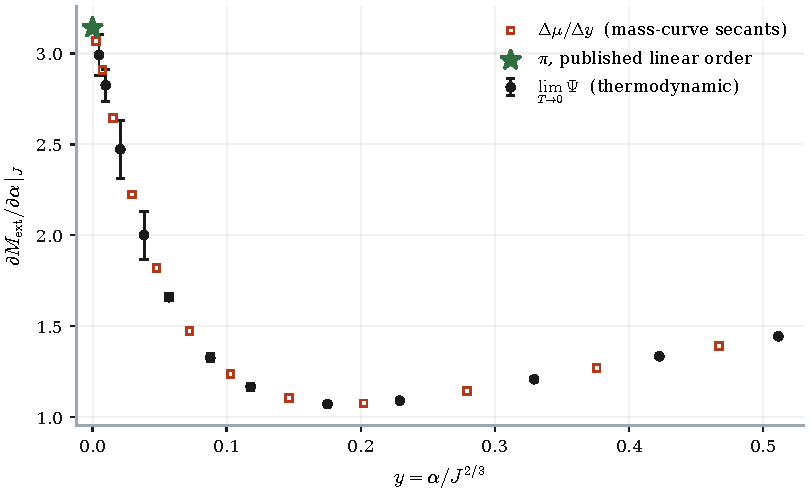
\includegraphics[width=.54\textwidth]{../manuscript/figures/fig-shift.pdf}\\[3pt]
 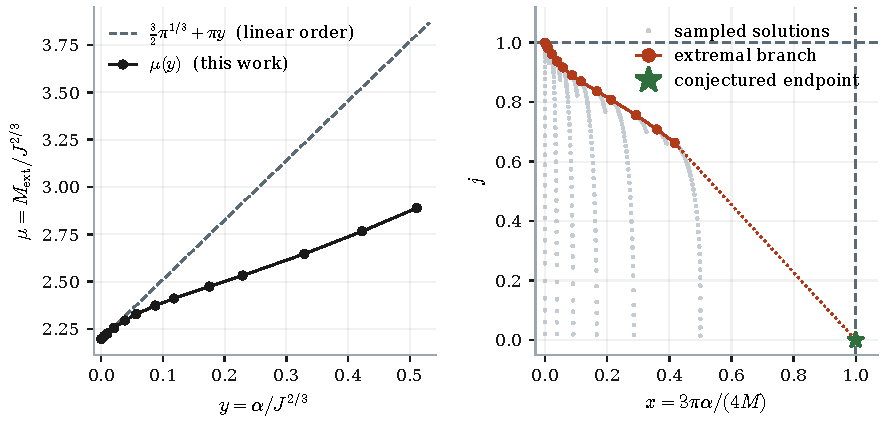
\includegraphics[width=.86\textwidth]{../manuscript/figures/fig-massext.pdf}
 \caption{Top: the measured slope against $y=\alpha/J^{2/3}$, with the
 published linear-order value $\pi$ as a star and secants of the mass curve as
 open squares. Bottom left: the extremal mass the slope integrates to, against
 the first-order line. Bottom right: the same branch in the $(x,j)$
 domain-of-existence plane of \aX{2303.12471}. Circles are $T=0$ intercepts of
 fits, not constructed solutions.}
\end{figure}

\paragraph{Three ways to read it.}
The result becomes less abstract when restated.
\begin{enumerate}\itemsep2pt
\item \emph{The spin bound, and the horizon.} By \eqref{eq:dictionary} a
 positive $\mu'$ is the same statement as a decreasing $j_\ext$, so the bound
 $j\le1$ reported in \aX{2303.12471} is the integrated form of the sign measured
 here pointwise. Equivalently, setting $T=0$ in the Smarr relation gives
 $\alpha\Psi_\ext=M_\ext-3\Omega_HJ$, so a positive slope is exactly
 $M_\ext>3\Omega_HJ$: the two sides coincide at $\alpha=0$, first order says the
 excess opens linearly, and the measurement says it keeps opening at a rate
 that falls and then recovers.
\item \emph{The geometry.} At fixed $T$ and $\Omega_i$ the Gibbs potential is
 the on-shell action per unit time, and the only explicit $\alpha$-dependence
 of that action is the Gauss--Bonnet term, so
 $\Psi=-(16\pi)^{-1}\int_\Sigma\sqrt{-g}\,\mathcal L_\GB\,\dd^4x$ over a
 stationary exterior slice: a positive $\Psi$ is a negative integrated
 Gauss--Bonnet density. Since the first law gives
 $\partial S/\partial\alpha|_{M,J}=-\Psi/T$, it is likewise a decrease of
 entropy at fixed mass and spin --- compatible with entropy per spin along the
 \emph{extremal} branch growing by a factor $\Nsigmagrowth$, because extremal
 states at fixed $J$ have different masses as $\alpha$ changes.
\item \emph{The turning point.} With $\omega=\Omega_HJ^{1/3}$, the same Smarr
 relation gives $3\omega=\mu-y\mu'$ and hence $3\omega'=-y\mu''$. For $y>0$ the
 inflection of the extremal mass is exactly the stationary point of $\omega$,
 and the minimum of the slope is a \emph{maximum} of $\omega$: the extremal
 horizon with the largest angular velocity in units of $J^{-1/3}$. That
 coupling is not otherwise distinguished, and is not a boundary of the domain
 of existence.
\end{enumerate}

\paragraph{Why the slope has to rise.}
The bound $M>3\pi\alpha/4$ is $\mu(y)>3\pi y/4$. If $\mu'$ stayed below some
$c<3\pi/4$ everywhere, then $\mu(y)\le\mu(0)+cy$, which violates the bound once
$y>\mu(0)/(3\pi/4-c)$. So $\mu'$ must return to at least
$3\pi/4=\Nslopeasymptote$, a value above every slope measured here: the
observed rise is required, not accidental. If the extremal branch also
terminates as conjectured in \aX{2303.12471}, the average slope tends to
$\Nslopeasymptote$. The sampled range stops well short of that --- the largest
$x$ reached on the extremal branch is $\Nxextlast$, against a conjectured
endpoint at $x=1$ --- so this is consistency, not evidence.

\section*{How far it can be trusted}

The response solve is the one step with no analytic counterpart, so it is
checked against four things that do not use it.

\begin{center}\small
\begin{tabular}{@{}lll@{}}
\toprule
check & what it tests & worst deviation \\
\midrule
Boulware--Deser static limit & $M,T,S,\Psi$ in closed form at finite $\alpha$ & $\Nstaticpsiworst$ \\
Published perturbative $\Psi_0(q)$ & the response at $\alpha=0$, at every spin & $\Noracleworst$ \\
Smarr relation as an equation for $\Psi$ & charges only: no Jacobian, no linear solve & $\Nsmarrpsiworst$ \\
On-shell Gauss--Bonnet action & curvature only: not even the charge extraction & $\Nonshellworst$ \\
Near-horizon entropy function & $S_\ext/J$ at finite coupling, algebraically & $\Nhorizonworst$ \\
First law in the spin direction & internal consistency of the observables & $\Nfirstlawworst$ \\
$G_{\mu\nu}+\alpha H_{\mu\nu}=0$ off-grid & equation closure, independent evaluator & $\Ntensorworst$ \\
Einstein extremal limits & $\mu(0)$ and $\Psi_\ext(0)$ against $\tfrac32\pi^{1/3}$, $\pi$ &
 $\Nmuzerodev$, $\Npsiextzerodev$ \\
Radial resolution, $\Nstudywalks$ full re-walks & the whole pipeline at two coarser $N$ & $\Nstudypsiworst$ \\
\bottomrule
\end{tabular}
\end{center}

The last two rows deserve comment. The Einstein limit is recovered from the
same continuation and extrapolation used at finite coupling, with the analytic
constants imposed nowhere; agreement there does not establish the error at
finite $y$. The resolution study re-ran the complete ascending sequence and the
complete $T=0$ extrapolation at two coarser base resolutions at every coupling,
and the intercept moves by less than the fit sensitivity in all $\Nstudywalks$
sequences --- which bounds the resolution effect but is not a convergence
proof, for three reasons named in the manuscript's appendix.

\paragraph{Limitations.}
The extrapolation is the leading one, and the bands around it are
sensitivities, not error bars. The coupling coverage is finite, the spin
coverage uneven, and the calculation is restricted to equal spins and to the
branch continuously connected to Myers--Perry; nothing here shows that branch
is unique, stable, or the lowest in mass at the same angular momenta. None of
the checks closes the gap that matters most: the mass-curve comparison shares
systematic errors with the potential, the near-horizon route determines entropy
rather than mass, and the Smarr and on-shell routes remove the response solve
from the chain but not the solutions. Finally, this is classical
Einstein--Gauss--Bonnet with the action \eqref{eq:action}. In a gravitational
effective field theory, terms beyond Gauss--Bonnet contribute at the same order
as the higher powers of $\alpha$ kept here, so the non-monotonic slope is not a
universal prediction of a derivative expansion.

\paragraph{One comparison that does not close.}
A separate reconstruction of the non-extremal family gives an outer ergosurface
radius $1.102101$ against the $1.104$ quoted in \aX{1010.0860}, at $\alpha=1/2$
in our convention. It is unresolved, recorded as a declared negative result
rather than absorbed into a tolerance, and not offered as evidence of an
erratum. It tests the metric functions away from the horizon and touches
neither the charge extraction, the response solve nor the extrapolation; the
near-horizon comparison that does test the same paper's coupling conversion
agrees to $\Npublishedstationarity$.

\section*{New, reproduced, and cited}

\emph{New here:} $\Psi$ measured on rotating solutions at finite coupling,
across the whole family and not only at its extremal end, with the sign change
it undergoes; the extremal slope obtained pointwise at $\Ncouplings$ couplings,
its minimum and subsequent rise resolved; the extremal mass curve it integrates
to, and the size of its departure from \eqref{eq:published}; the reading of
$\Psi$ as an on-shell Gauss--Bonnet action, tested against the response on
$\Nonshellstates$ archived solutions; and the identification of the slope
minimum with the maximum of $\Omega_HJ^{1/3}$.

\emph{Reproduced rather than new:} the equal-spin family of \aX{1010.0860} and
its profiles; the closed-form static solution; the $\mathcal O(\alpha)$
potential implied by \aX{2405.04576} and the first-order extremal mass $\pi$ of
\aX{2009.00015}; the near-horizon extremal entropy of \aX{1010.0860}; and the
extremal branch itself, which \aX{2303.12471} constructs directly and this work
reaches by extrapolation, with its bounds $j\le1$ and $x<1$.

\emph{Cited, not reproduced:} the Myers--Perry and Boulware--Deser solutions
(oracles, every closed form checked against the solver, but not rederived),
Lovelock's theorem, the Wald and Jacobson--Myers entropy formulae, Sen's
entropy function formalism, the covariant phase space derivation of the
extended $\alpha$-term, and the Goon--Penco universality claim --- of which
only the first-law identity is used, and that is rederived.

\section*{The apparatus}

One discipline shaped the repository more than any other: \textbf{no number
that appears in the paper is typed into the paper}. Every figure, table and
quoted quantity is generated from the recorded measurement into
\texttt{numbers.tex} and read back as a macro, so the PDF, the figures, the
tables and the data cannot disagree: rebuilding either reproduces them or
fails. This document draws on the same file.

Around that sit the checks that make a claim auditable rather than merely
stated. A static checker verifies that every generated quantity is used and
every used one generated, that no literal decimal survives in the prose, and
that every citation resolves. Each result carries a provenance record naming
its command, inputs and their hashes, audited against the bytes on disk, with
the two exceptions it cannot resolve documented rather than silenced. Failed
checks are declared in \texttt{artifacts/limitations.json}, and a test asserts
that the declared failures still match the actual ones, so the list cannot grow
into a way of muting the audit.

Two lessons are worth recording. Re-running the same boundary-value problem on
a different linear-algebra stack moved an extrapolated intercept by more than
either genuine resolution change at the same coupling: the walk is adaptive, so
a different BLAS changes which states pass the acceptance gate and therefore
which states get fitted. And the quadrature for the on-shell integral
\emph{cannot} be refined --- $\mathcal L_\GB$ is a cancellation decaying like
$r^{-8}$ while the compactification amplifies what survives, so past about
eighty nodes the answer degrades and then diverges. In both, the obvious
convergence diagnostic measures something other than what it appears to.

\end{document}
